% !TeX root = ../main.tex
\documentclass[./../main.tex]{subfiles}

\begin{document}

\subsection{Mô hình ca sử dụng}

\subsubsection{Sơ đồ chính}

Hình \ref{fig:use_case_diagram} mô tả tác nhân và ca sử dụng chính của hệ thống.

\begin{figure}[h!]
  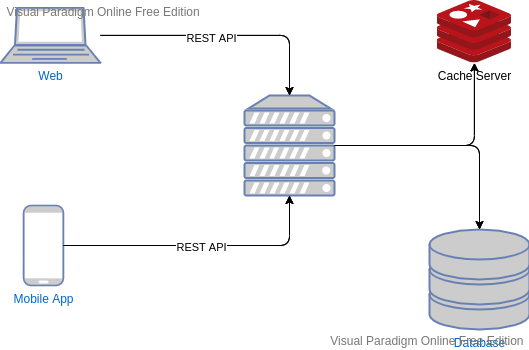
\includegraphics[width=\linewidth]{./images/image4.png}
  \caption{Mô hình ca sử dụng}
  \label{fig:use_case_diagram}
\end{figure}

\subsubsection{Tác nhân của hệ thống}

\begin{itemize}
  \item
    \begin{quote}
    \textbf{Người dùng} là người đã có tài khoản để truy cập vào hệ thống.
    \end{quote}
  \item
    \begin{quote}
    \textbf{Sinh viên} là người dùng hệ thống, sử dụng hệ thống để đăng ký
    thực tập, nộp báo cáo và xem kết quả thực tập.
    \end{quote}
  \item
    \begin{quote}
    \textbf{Giảng viên} là người dùng hệ thống, sử dụng hệ thống để quản
    lý và chấm điểm cho danh sách sinh viên đang hướng dẫn.
    \end{quote}
  \item
    \begin{quote}
    \textbf{Đối tác} là người dùng hệ thống, sử dụng hệ thống để quản lý
    bài đăng tuyển dụng, danh sách yêu cầu thực tập và danh sách sinh viên
    đang thực tập tại đơn vị.
    \end{quote}
  \item
    \begin{quote}
    \textbf{Quản trị viên Khoa} là người dùng hệ thống, sử dụng hệ thống
    để quản lý danh sách các kỳ thực tập, danh sách sinh viên, đơn vị thực
    tập, giảng viên theo từng kỳ và thông tin cá nhân của các đối tượng
    đó.
    \end{quote}
  \item
    \begin{quote}
    \textbf{Quản trị viên} là người dùng hệ thống, sử dụng hệ thống để
    quản lý danh sách các Khoa, danh sách lớp và quản lý tài khoản người
    dùng hệ thống.
    \end{quote}
  \end{itemize}

  \subsection{Yêu cầu chức năng}

  \hypertarget{ux111ux103ng-nhux1eadp-hux1ec7-thux1ed1ng}{%
  \subsubsection{Đăng nhập hệ
  thống}\label{ux111ux103ng-nhux1eadp-hux1ec7-thux1ed1ng}}
  
  Người dùng cung cấp email và mật khẩu để truy cập vào hệ thống.
  
  Ngoài đăng nhập bằng email và mật khẩu, người dùng có thể đăng nhập bằng
  LDAP và Google.
  
  \hypertarget{ux111ux1eb7t-lux1ea1i-mux1eadt-khux1ea9u}{%
  \subsubsection{Đặt lại mật
  khẩu}\label{ux111ux1eb7t-lux1ea1i-mux1eadt-khux1ea9u}}
  
  Người dùng sử dụng chức năng này khi quên mật khẩu tài khoản. Hệ thống
  sẽ yêu cầu người dùng nhập email VNU và gửi một đường link đặt lại mật
  khẩu cho người dùng.
  
  \hypertarget{ux111ux1ed5i-mux1eadt-khux1ea9u}{%
  \subsubsection{Đổi mật khẩu}\label{ux111ux1ed5i-mux1eadt-khux1ea9u}}
  
  Người dùng có thể đổi mật khẩu.
  
  \hypertarget{chux1ec9nh-sux1eeda-thuxf4ng-tin-cuxe1-nhuxe2n}{%
  \subsubsection{Chỉnh sửa thông tin cá
  nhân}\label{chux1ec9nh-sux1eeda-thuxf4ng-tin-cuxe1-nhuxe2n}}
  
  Người dùng \textbf{sinh viên}, \textbf{giảng viên} và \textbf{đối tác}
  có thể chỉnh sửa thông tin cá nhân của bản thân.
  
  \hypertarget{xem-thuxf4ng-tin-buxe0i-ux111ux103ng}{%
  \subsubsection{Xem thông tin bài
  đăng}\label{xem-thuxf4ng-tin-buxe0i-ux111ux103ng}}
  
  Người dùng \textbf{sinh viên} có thể xem thông tin cơ bản về bài đăng,
  bao gồm:
  
  \begin{itemize}
  \item
    \begin{quote}
    Tiêu đề bài viết
    \end{quote}
  \item
    \begin{quote}
    Thời gian đăng
    \end{quote}
  \item
    \begin{quote}
    Tên công ty tuyển dụng
    \end{quote}
  \item
    \begin{quote}
    Thông tin liên lạc của công ty
    \end{quote}
  \item
    \begin{quote}
    Thông tin về vị trí, số lượng, thời hạn tuyển dụng
    \end{quote}
  \item 
    \begin{quote}
    Nội dung bài viết
    \end{quote}
  \end{itemize}
  
  \hypertarget{xem-quy-chux1ebf-thux1ef1c-tux1eadp}{%
  \subsubsection{Xem quy chế thực
  tập}\label{xem-quy-chux1ebf-thux1ef1c-tux1eadp}}
  
  Người dùng \textbf{sinh viên} có thể đọc về quy chế thực tập và hướng
  dẫn sử dụng hệ thống.
  
  \hypertarget{ux111ux103ng-kuxfd-thux1ef1c-tux1eadp-vux1edbi-cuxf4ng-ty-liuxean-kux1ebft}{%
  \subsubsection{Đăng ký thực tập với công ty liên
  kết}\label{ux111ux103ng-kuxfd-thux1ef1c-tux1eadp-vux1edbi-cuxf4ng-ty-liuxean-kux1ebft}}
  
  Người dùng \textbf{sinh viên} đang trong thời gian thực tập chuyên ngành
  có thể tìm kiếm và đăng ký thực tập với công ty liên kết. Nếu công ty
  tìm kiếm không thuộc công ty liên kết, người dùng cần đăng ký thực tập
  với công ty ngoài.
  
  \hypertarget{ux111ux103ng-kuxfd-thux1ef1c-tux1eadp-vux1edbi-cuxf4ng-ty-ngouxe0i}{%
  \subsubsection{Đăng ký thực tập với công ty
  ngoài}\label{ux111ux103ng-kuxfd-thux1ef1c-tux1eadp-vux1edbi-cuxf4ng-ty-ngouxe0i}}
  
  Người dùng \textbf{sinh viên} đang trong thời gian thực tập chuyên ngành
  có thể tìm kiếm và yêu cầu đăng ký thực tập với công ty ngoài. Các yêu
  cầu này cần được Khoa xét duyệt và có thể bị từ chối.
  
  \begin{itemize}
  \item
    \begin{quote}
    Nếu công ty đã có trong cơ sở dữ liệu thì người dùng sinh viên có thể
    gửi yêu cầu thực tập và đợi kết quả xét duyệt từ Khoa.
    \end{quote}
  \item
    \begin{quote}
    Nếu công ty chưa có trong cơ sở dữ liệu thì người dùng sinh viên phải
    gửi thông tin công ty cho Khoa xét duyệt và đợi kết quả từ Khoa trước
    khi gửi yêu cầu thực tập.
    \end{quote}
  \end{itemize}
  
  \hypertarget{ux111ux103ng-kuxfd-phux1ecfng-vux1ea5n-tux1eeb-buxe0i-ux111ux103ng}{%
  \subsubsection{Đăng ký phỏng vấn từ bài
  đăng}\label{ux111ux103ng-kuxfd-phux1ecfng-vux1ea5n-tux1eeb-buxe0i-ux111ux103ng}}
  
  Người dùng \textbf{sinh viên} chưa đi thực tập tại đơn vị nào có thể
  đăng ký phỏng vấn vào các công ty đang đăng bài tuyển dụng.
  
  \hypertarget{xem-thuxf4ng-tin-thux1ef1c-tux1eadp}{%
  \subsubsection{Xem thông tin thực
  tập}\label{xem-thuxf4ng-tin-thux1ef1c-tux1eadp}}
  
  Người dùng \textbf{sinh viên} có thể xem thông tin của mình trong kỳ
  thực tập. Thông tin bao gồm:
  
  \begin{itemize}
  \item
    \begin{quote}
    Công ty đã chọn
    \end{quote}
  \item
    \begin{quote}
    Thông tin của giảng viên hướng dẫn
    \end{quote}
  \item
    \begin{quote}
    Danh sách công ty đã đỗ và chưa đỗ phỏng vấn
    \end{quote}
  \end{itemize}
  
  \hypertarget{chux1ecdn-cuxf4ng-ty-ux111ux1ec3-thux1ef1c-tux1eadp}{%
  \subsubsection{Chọn công ty để thực
  tập}\label{chux1ecdn-cuxf4ng-ty-ux111ux1ec3-thux1ef1c-tux1eadp}}
  
  Nếu đỗ phỏng vấn nhiều công ty, người dùng \textbf{sinh viên} bắt buộc
  phải chọn một công ty để thực tập.
  
  \hypertarget{nux1ed9p-buxe1o-cuxe1o-thux1ef1c-tux1eadp}{%
  \subsubsection{Nộp báo cáo thực
  tập}\label{nux1ed9p-buxe1o-cuxe1o-thux1ef1c-tux1eadp}}
  
  Người dùng \textbf{sinh viên} có thể nộp báo cáo thực tập để được giảng
  viên hướng dẫn nhận xét và chấm điểm.
  
  \hypertarget{tux1ea3i-luxean-cv}{%
  \subsubsection{Tải lên CV}\label{tux1ea3i-luxean-cv}}
  
  Người dùng \textbf{sinh viên} có thể tải lên CV. CV này sẽ có thể được
  xem bởi công ty và giảng viên hướng dẫn trong quá trình chấp nhận và từ
  chối yêu cầu thực tập.
  
  \hypertarget{xem-thux1ed1ng-kuxea-dux1eef-liux1ec7u-truxean-hux1ec7-thux1ed1ng}{%
  \subsubsection{Xem thống kê dữ liệu trên hệ
  thống}\label{xem-thux1ed1ng-kuxea-dux1eef-liux1ec7u-truxean-hux1ec7-thux1ed1ng}}
  
  Người dùng \textbf{giảng viên, đối tác, quản trị viên Khoa, quản trị
  viên} có thể xem thống kê dữ liệu trên hệ thống.
  
  \hypertarget{xem-danh-suxe1ch-sinh-viuxean-ux111ang-hux1b0ux1edbng-dux1eabn}{%
  \subsubsection{Xem danh sách sinh viên đang hướng
  dẫn}\label{xem-danh-suxe1ch-sinh-viuxean-ux111ang-hux1b0ux1edbng-dux1eabn}}
  
  Người dùng \textbf{giảng viên} có thể xem danh sách sinh viên đang hướng
  dẫn thực tập và thông tin cá nhân của những sinh viên đó.
  
  \hypertarget{xem-buxe1o-cuxe1o-thux1ef1c-tux1eadp-cux1ee7a-sinh-viuxean}{%
  \subsubsection{Xem báo cáo thực tập của sinh
  viên}\label{xem-buxe1o-cuxe1o-thux1ef1c-tux1eadp-cux1ee7a-sinh-viuxean}}
  
  Người dùng \textbf{giảng viên} có thể xem và tải về báo cáo thực tập của
  sinh viên mình đang hướng dẫn.
  
  \hypertarget{chux1ea5m-ux111iux1ec3m-cho-sinh-viuxean}{%
  \subsubsection{Chấm điểm cho sinh
  viên}\label{chux1ea5m-ux111iux1ec3m-cho-sinh-viuxean}}
  
  Người dùng \textbf{giảng viên} có thể bổ sung đầu điểm giữa kỳ và cuối
  kỳ cho sinh viên mình đang hướng dẫn thông qua biểu mẫu nộp điểm. Hai
  đầu điểm này sẽ được sử dụng để tính ra điểm tổng kết cuối cùng.
  
  \hypertarget{quux1ea3n-luxfd-buxe0i-ux111ux103ng-cux1ee7a-muxecnh}{%
  \subsubsection{Quản lý bài đăng của
  mình}\label{quux1ea3n-luxfd-buxe0i-ux111ux103ng-cux1ee7a-muxecnh}}
  
  Người dùng \textbf{đối tác} có thể:
  
  \begin{itemize}
  \item
    \begin{quote}
    Xem, tìm kiếm bài đăng
    \end{quote}
  \item
    \begin{quote}
    Chỉnh sửa và tạo mới bài đăng để tuyển dụng thực tập sinh.
    \end{quote}
  \end{itemize}
  
  \hypertarget{quux1ea3n-luxfd-yuxeau-cux1ea7u-thux1ef1c-tux1eadp-cux1ee7a-sinh-viuxean}{%
  \subsubsection{Quản lý yêu cầu thực tập của sinh
  viên}\label{quux1ea3n-luxfd-yuxeau-cux1ea7u-thux1ef1c-tux1eadp-cux1ee7a-sinh-viuxean}}
  
  Người dùng \textbf{đối tác} có thể:
  
  \begin{itemize}
  \item
    \begin{quote}
    Xem, lọc, tìm kiếm sinh viên
    \end{quote}
  \item
    \begin{quote}
    Chấp nhận yêu cầu sinh viên
    \end{quote}
  \item
    \begin{quote}
    Từ chối yêu cầu của sinh viên
    \end{quote}
  \end{itemize}
  
  \hypertarget{quux1ea3n-luxfd-sinh-viuxean-ux111ang-thux1ef1c-tux1eadp-tux1ea1i-cuxf4ng-ty}{%
  \subsubsection{Quản lý sinh viên đang thực tập tại công
  ty}\label{quux1ea3n-luxfd-sinh-viuxean-ux111ang-thux1ef1c-tux1eadp-tux1ea1i-cuxf4ng-ty}}
  
  Người dùng \textbf{đối tác} có thể xem, lọc, tìm kiếm sinh viên.
  
  \hypertarget{quux1ea3n-luxfd-kux1ef3-thux1ef1c-tux1eadp}{%
  \subsubsection{Quản lý kỳ thực
  tập}\label{quux1ea3n-luxfd-kux1ef3-thux1ef1c-tux1eadp}}
  
  Người dùng \textbf{quản trị viên Khoa} có thể tạo kỳ thực tập mới. Một
  kỳ thực tập bao gồm những thông tin sau:
  
  \begin{quote}
  \textbf{Danh sách công ty cho phép đăng ký thực tập} Người dùng sinh
  viên chỉ có thể đăng ký thực tập với các công ty nằm trong danh sách
  này. Khi tạo, danh sách các công ty đối tác còn hiệu lực của khoa này sẽ
  được tự động thêm vào danh sách cho phép đăng ký của kỳ thực tập. Ngoài
  ra, quản trị viên cũng có thể thêm hoặc xóa bỏ công ty trong danh sách
  cho phép một cách thủ công.
  
  \textbf{Thời hạn thực tập} Khoảng thời gian 2-3 tháng mà trong đó sinh
  viên được phép đăng ký thực tập.
  \end{quote}
  
  Khi tạo 1 kỳ thực tập mới, cho phép tạo luôn danh sách các công ty đối
  tác được chấp nhận trong kỳ này bằng 2 cách: chọn các công ty đã có
  trong CSDL và bổ sung các công ty mới. Sau khi có danh sách này, các bài
  đăng sẽ \textbf{tự động được sinh ra} (nội dung trống) để cho sinh viên
  đăng ký. Sau khi có danh sách này, hệ thống sẽ tự động hiển thị form
  đăng ký cho tất cả công ty trong kỳ thực tập.
  
  \hypertarget{quux1ea3n-luxfd-danh-suxe1ch-sinh-viuxean-ux111ang-thux1ef1c-tux1eadp}{%
  \subsubsection{Quản lý danh sách sinh viên đang thực
  tập}\label{quux1ea3n-luxfd-danh-suxe1ch-sinh-viuxean-ux111ang-thux1ef1c-tux1eadp}}
  
  Người dùng \textbf{quản trị viên Khoa} có thể:
  
  \begin{itemize}
  \item
    \begin{quote}
    Xem danh sách sinh viên đang thực tập
    \end{quote}
  \item
    \begin{quote}
    Lọc, tìm kiếm và sắp xếp danh sách sinh viên thực tập
    \end{quote}
  \item
    \begin{quote}
    Tải danh sách sinh viên sau khi lọc
    \end{quote}
  \item
    \begin{quote}
    Gửi thông báo trúng tuyển hoặc thông báo trượt phỏng vấn
    \end{quote}
  \end{itemize}

  \hypertarget{quux1ea3n-luxfd-danh-suxe1ch-ux111ux1ed1i-tuxe1c-trong-kux1ef3-thux1ef1c-tux1eadp}{%
  \subsubsection{Quản lý danh sách đối tác trong kỳ thực
  tập}\label{quux1ea3n-luxfd-danh-suxe1ch-ux111ux1ed1i-tuxe1c-trong-kux1ef3-thux1ef1c-tux1eadp}}
  
  Người dùng \textbf{quản trị viên Khoa} có thể:
  
  \begin{itemize}
  \item
    \begin{quote}
    Xem danh sách đối tác trong kỳ thực tập
    \end{quote}
  \item
    \begin{quote}
    Lọc, tìm kiếm và sắp xếp danh sách đối tác
    \end{quote}
  \item
    \begin{quote}
    Chấp nhận/từ chối công ty trong kỳ thực tập
    \end{quote}
  \end{itemize}
  
  \hypertarget{quux1ea3n-luxfd-buxe0i-ux111ux103ng-cux1ee7a-tux1ea5t-cux1ea3-ux111ux1ed1i-tuxe1c-trong-kux1ef3-thux1ef1c-tux1eadp}{%
  \subsubsection{Quản lý bài đăng của tất cả đối tác trong kỳ thực
  tập}\label{quux1ea3n-luxfd-buxe0i-ux111ux103ng-cux1ee7a-tux1ea5t-cux1ea3-ux111ux1ed1i-tuxe1c-trong-kux1ef3-thux1ef1c-tux1eadp}}
  
  Người dùng \textbf{quản trị viên khoa} có thể:
  
  \begin{itemize}
  \item
    \begin{quote}
    Xem, tìm kiếm bài đăng
    \end{quote}
  \item
    \begin{quote}
    Tạo và chỉnh sửa tất cả bài đăng trong khoa của mình.
    \end{quote}
  \item
    \begin{quote}
    Ngoài ra, có thể xét duyệt bài đăng của đối tác. Chỉ những bài đăng
    được duyệt mới được hiển thị cho sinh viên.
    \end{quote}
  \end{itemize}
  
  \hypertarget{quux1ea3n-luxfd-giux1ea3ng-viuxean-hux1b0ux1edbng-dux1eabn-trong-kux1ef3-thux1ef1c-tux1eadp}{%
  \subsubsection{Quản lý giảng viên hướng dẫn trong kỳ thực
  tập}\label{quux1ea3n-luxfd-giux1ea3ng-viuxean-hux1b0ux1edbng-dux1eabn-trong-kux1ef3-thux1ef1c-tux1eadp}}
  
  Người dùng \textbf{quản trị viên khoa} có thể thêm / sửa giảng viên
  hướng dẫn cho sinh viên. Sau khi thêm xong, người này có thể gửi danh
  sách sinh viên hướng dẫn tới mail của từng giảng viên.
  
  \hypertarget{quux1ea3n-luxfd-danh-suxe1ch-sinh-viuxean}{%
  \subsubsection{Quản lý danh sách sinh
  viên}\label{quux1ea3n-luxfd-danh-suxe1ch-sinh-viuxean}}
  
  Người dùng \textbf{quản trị viên Khoa} có thể xem, lọc, tìm kiếm thông
  tin cá nhân của sinh viên trong Khoa.
  
  \hypertarget{quux1ea3n-luxfd-danh-suxe1ch-ux111ux1ed1i-tuxe1c}{%
  \subsubsection{Quản lý danh sách đối
  tác}\label{quux1ea3n-luxfd-danh-suxe1ch-ux111ux1ed1i-tuxe1c}}
  
  Người dùng \textbf{quản trị viên Khoa} có thể:
  
  \begin{itemize}
  \item
    \begin{quote}
    Xem, tìm kiếm, lọc danh sách công ty liên kết và công ty ngoài trong
    Khoa
    \end{quote}
  \item
    \begin{quote}
    Thêm và sửa liên hệ cho công ty
    \end{quote}
  \end{itemize}
  
  \hypertarget{quux1ea3n-luxfd-danh-suxe1ch-giux1ea3ng-viuxean}{%
  \subsubsection{Quản lý danh sách giảng
  viên}\label{quux1ea3n-luxfd-danh-suxe1ch-giux1ea3ng-viuxean}}
  
  Người dùng \textbf{quản trị viên Khoa} có thể xem, tìm kiếm danh sách
  người dùng giảng viên trong Khoa.
  
  \hypertarget{quux1ea3n-luxfd-ngux1b0ux1eddi-duxf9ng}{%
  \subsubsection{Quản lý người
  dùng}\label{quux1ea3n-luxfd-ngux1b0ux1eddi-duxf9ng}}
  
  Người dùng \textbf{quản trị viên} có thể thêm / sửa thông tin người dùng
  trên hệ thống. Thông tin người dùng bao gồm:
  
  \begin{itemize}
  \item
    \begin{quote}
    Thông tin cá nhân: tên, email, ngày sinh, mã số sinh viên, \ldots{}
    \end{quote}
  \item
    \begin{quote}
    Thông tin đăng nhập: tên đăng nhập, mật khẩu, ...
    \end{quote}
  \end{itemize}
  
  \hypertarget{quux1ea3n-luxfd-danh-suxe1ch-khoa}{%
  \subsubsection{Quản lý danh sách
  khoa}\label{quux1ea3n-luxfd-danh-suxe1ch-khoa}}
  
  Người dùng \textbf{quản trị viên} có thể thêm / sửa / xóa Khoa và quản
  lý tài khoản quản trị viên cho Khoa đó.
  
  \hypertarget{quux1ea3n-luxfd-danh-suxe1ch-lux1edbp}{%
  \subsubsection{Quản lý danh sách
  lớp}\label{quux1ea3n-luxfd-danh-suxe1ch-lux1edbp}}
  
  Người dùng \textbf{quản trị viên} có thể thêm / sửa /xóa lớp.

\subsection{Yêu cầu phi chức năng}

\hypertarget{tuxednh-khux1ea3-dux1ee5ng}{%
\subsubsection{Tính khả dụng}\label{tuxednh-khux1ea3-dux1ee5ng}}

Người dùng thuộc đối tượng sinh viên, giảng viên cần có thể thực hiện
chức năng của hệ thống trong không quá 10 phút.

\hypertarget{ux111ux1ed9-tin-cux1eady}{%
\subsubsection{Độ tin cậy}\label{ux111ux1ed9-tin-cux1eady}}

Hệ thống không bị sập do lỗi phần mềm. Thời gian uptime của server sẽ
phụ thuộc vào bên quản lý hạ tầng.

\hypertarget{hiux1ec7u-suux1ea5t}{%
\subsubsection{Hiệu suất}\label{hiux1ec7u-suux1ea5t}}

Phần này mô tả các yêu cầu phi chức năng liên quan đến hiệu suất của hệ
thống.

Hệ thống cần có sức chứa như sau:

\begin{itemize}
\item
  \begin{quote}
  Hỗ trợ tối thiểu 500 yêu cầu đồng thời
  \end{quote}
\item
  \begin{quote}
  Hỗ trợ tối thiểu 30000 thành viên
  \end{quote}
\end{itemize}

Hệ thống cần phải thỏa mãn những yêu cầu sau:

\begin{itemize}
\item
  \begin{quote}
  Hoàn thành 95\% yêu cầu trong thời gian dưới 2 giây.
  \end{quote}
\item
  \begin{quote}
  Hoàn thành 99\% yêu cầu trong thời gian dưới 5 giây.
  \end{quote}
\end{itemize}

\hypertarget{khux1ea3-nux103ng-truy-cux1eadp}{%
\subsubsection{Khả năng truy cập}\label{khux1ea3-nux103ng-truy-cux1eadp}}

Hệ thống cần phải tuân thủ nguyên tắc về khả năng truy cập của
\href{https://www.w3.org/WAI/fundamentals/accessibility-principles/}{\underline{W3C}},
ví dụ như:

\begin{itemize}
\item
  \begin{quote}
  Cung cấp mô tả bằng văn bản cho nội dung đa phương tiện
  \end{quote}
\item
  \begin{quote}
  Có thể điều hướng và sử dụng trang web chỉ bằng bàn phím
  \end{quote}
\item
  \begin{quote}
  Hiển thị thông tin với phông chữ và màu sắc có độ tương phản cao
  \end{quote}
\end{itemize}

\hypertarget{tuxednh-bux1ea3o-mux1eadt}{%
\subsubsection{Tính bảo mật}\label{tuxednh-bux1ea3o-mux1eadt}}

Hệ thống cần:

\begin{itemize}
\item
  \begin{quote}
  Đưa ra phương pháp để tránh lỗ hổng bảo mật trên ứng dụng Web như đề
  xuất của
  \href{https://owasp.org/www-project-top-ten/}{\underline{OWASP}}.
  \end{quote}
\item
  \begin{quote}
  Cài đặt tính năng logging mỗi khi có thay đổi được thực hiện trong cơ
  sở dữ liệu (thêm kỳ thực tập, xóa kỳ thực tập, \ldots).
  \end{quote}
\end{itemize}

\hypertarget{giao-diux1ec7n}{%
\subsubsection{Giao diện}\label{giao-diux1ec7n}}

Giao diện sản phẩm cần phải thoả mãn yêu cầu về khả năng truy cập. Ngoài
ra, giao diện cần hỗ trợ nhiều kích cỡ màn hình khác nhau và tuân thủ
theo nguyên tắc thiết kế của trường Đại Học Quốc Gia Hà Nội.

\hypertarget{bux1ea3o-truxec-vuxe0-lux1b0u-chuyux1ec3n}{%
\subsubsection{Bảo trì và lưu
chuyển}\label{bux1ea3o-truxec-vuxe0-lux1b0u-chuyux1ec3n}}

Hệ thống cần cung cấp bộ ca kiểm thử đơn vị, tích hợp và hệ thống để sau
này có thể dễ dàng bảo trì và nâng cấp phần mềm.

\subsection{Đặc tả ca sử dụng}

\hypertarget{ux111ux103ng-nhux1eadp-hux1ec7-thux1ed1ng-1}{%
\subsubsection{Đăng nhập hệ
thống}\label{ux111ux103ng-nhux1eadp-hux1ec7-thux1ed1ng-1}}

\paragraph*{Mô tả tóm tắt} ~\\

Người dùng đăng nhập vào hệ thống với tài khoản được cấp.

\paragraph*{Luồng sự kiện} ~\\

\emph{Luồng chính:} Ca sử dụng này bắt đầu khi người dùng mong muốn đăng
nhập vào hệ thống.

\begin{table}[H]
  \begin{tabular}{|p{.4\textwidth}|p{.3\textwidth}|p{.3\textwidth}|}
  \hline
  \textbf{Hành động}                   & \textbf{Hệ thống phản hồi}                                                    & \textbf{Dữ liệu}              \\ \hline
Người dùng truy cập trang đăng nhập. & Hệ thống yêu cầu người dùng nhập email và mật khẩu.                           &                               \\ \hline
Người dùng điền các thông tin.       & Hệ thống kiểm định thông tin và điều hướng người dùng vào hệ thống theo Role. & Email và mật khẩu người dùng. \\ \hline
  \end{tabular}
\end{table}

\emph{Luồng thay thế:}

\begin{itemize}
\item
  \begin{quote}
  Tại bước 3: Thay vì đăng nhập bằng email và mật khẩu, người dùng yêu
  cầu đăng nhập bằng Google, hệ thống điều hướng và mở một trang đăng
  nhập bằng tài khoản Google.
  \end{quote}
\end{itemize}

\emph{Luồng ngoại lệ:}

\begin{itemize}
\item
  \begin{quote}
  Tại bước 3: Người dùng điền thiếu hoặc sai thông tin, hệ thống yêu cầu
  nhập lại.
  \end{quote}
\item
  \begin{quote}
  Tại bước 4: Hệ thống kiểm định thông tin đăng nhập sai, hệ thống hiển
  thị thông tin lỗi, yêu cầu nhập lại. Người dùng có thể tiếp tục lặp
  lại luồng sự kiện hoặc thoát khỏi trang đăng nhập.
  \end{quote}
\end{itemize}

\paragraph*{Yêu cầu đặc biệt} ~\\

Người dùng đã có tài khoản trong hệ thống.

\paragraph*{Điều kiện đầu} ~\\

Không có.

\paragraph*{Điều kiện cuối} ~\\

Nếu ca sử dụng thành công, người dùng đã được đăng nhập vào hệ thống,
ngược lại, trạng thái hệ thống không thay đổi.

\paragraph*{Các vấn đề mở} ~\\

Không có.

\end{document}